% !TeX program = xelatex
\documentclass[a4paper,10pt]{article}

% ============================================================================
% សន្លឹកកិច្ចការសិស្សបំពេញចន្លោះ ស-ខ្មៅ និងប្លង់ក្ដារខៀន/ចម្លើយគ្រូ (គ្មាន LCD / គ្មានកន្ត្រៃ)
% មេរៀនទី៥ (១.១--១.៣)៖ សញ្ញាណឯកធា ឯកធាដូចគ្នា និងដឺក្រេនៃឯកធា — ត្រូវគ្នានឹង LS_Plan_ALG51.tex
% ============================================================================
\usepackage[a4paper, left=1.0cm, right=1.0cm, top=0.75cm, bottom=1.00cm, footskip=0.52cm]{geometry}
\usepackage{amsmath}
\usepackage{unicode-math}
\usepackage{fontspec}
\usepackage{array, colortbl}
\usepackage[table]{xcolor}
\usepackage{enumitem}
\usepackage{pifont}
\usepackage{fancyhdr}
\usepackage{lastpage}
\usepackage{tikz}
\usepackage[most]{tcolorbox}
\usetikzlibrary{calc, arrows.meta, decorations.pathreplacing, positioning, babel}

\makeatletter
\let\@expl@@@mark@update@singlecol@structures@@\relax
\makeatother

\providecommand{\NGSFindFonts}{%
  \IfFileExists{C:/Windows/Fonts/cambria.ttc}{%
    \def\NGSSysPath{C:/Windows/Fonts/}%
    \def\NGSUserPath{C:/Users/KIT/AppData/Local/Microsoft/Windows/Fonts/}%
  }{%
    \IfFileExists{./fonts/KhmerOSsiemreap.ttf}{\def\NGSSysPath{./fonts/}\def\NGSUserPath{./fonts/}}{%
    \IfFileExists{../fonts/KhmerOSsiemreap.ttf}{\def\NGSSysPath{../fonts/}\def\NGSUserPath{../fonts/}}{%
    \IfFileExists{../../fonts/KhmerOSsiemreap.ttf}{\def\NGSSysPath{../../fonts/}\def\NGSUserPath{../../fonts/}}{%
    \IfFileExists{../../../fonts/KhmerOSsiemreap.ttf}{\def\NGSSysPath{../../../fonts/}\def\NGSUserPath{../../../fonts/}}{%
    \IfFileExists{../../../../fonts/KhmerOSsiemreap.ttf}{\def\NGSSysPath{../../../../fonts/}\def\NGSUserPath{../../../../fonts/}}{%
    \IfFileExists{../../../../../fonts/KhmerOSsiemreap.ttf}{\def\NGSSysPath{../../../../../fonts/}\def\NGSUserPath{../../../../../fonts/}}{%
    \IfFileExists{../../../../../../fonts/KhmerOSsiemreap.ttf}{\def\NGSSysPath{../../../../../../fonts/}\def\NGSUserPath{../../../../../../fonts/}}{%
      \def\NGSSysPath{../../../../../../../fonts/}\def\NGSUserPath{../../../../../../../fonts/}%
    }}}}}}}%
  }%
}
\NGSFindFonts

\setmathfont[Path={\NGSSysPath}, FontIndex=1, Scale=1.02]{cambria.ttc}
\defaultfontfeatures{Ligatures=TeX}

\setmainfont[
  Path={\NGSUserPath}, Extension=.ttf, Script=Khmer,
  BoldFont={KhmerOSsiemreap}, BoldFeatures={FakeBold=1.8},
  ItalicFont={KhmerOSsiemreap}, ItalicFeatures={FakeSlant=0.25},
  BoldItalicFont={KhmerOSsiemreap}, BoldItalicFeatures={FakeBold=1.8, FakeSlant=0.25}
]{KhmerOSsiemreap}

\newfontfamily\muol[Path={\NGSUserPath}, Extension=.ttf, Script=Khmer]{KhmerOSmuollight}
\newfontfamily\TimesEn[Path={\NGSSysPath}, Extension=.ttf, BoldFont={timesbd}, ItalicFont={timesi}, BoldItalicFont={timesbi}]{times}
\newfontfamily\CalibriFont[Path={\NGSSysPath}, Extension=.ttf]{calibri}

\XeTeXlinebreaklocale "km"
\XeTeXlinebreakskip = 0pt plus 1pt minus 0.1pt

\definecolor{panelgray}{gray}{0.94}
\definecolor{headgray}{gray}{0.85}

\pagestyle{fancy}
\fancyhf{}
\renewcommand{\headrulewidth}{0pt}
\fancyfoot[L]{\fontsize{7.4pt}{9.5pt}\selectfont អនុវិទ្យាល័យព្រះក្រសាំង \en{|} គ្រូ៖ ហុក ប៊ុនថែន \en{|} មេរៀនទី៥ (១.១--១.៣) ឯកធា \en{|} ថ្ងៃសុក្រ ទី៤ ខែធ្នូ ឆ្នាំ២០២៦}
\fancyfoot[R]{\fontsize{7.8pt}{10pt}\selectfont ទំព័រ \en{\thepage\ / \pageref{LastPage}}}

\setlength{\parindent}{0pt}
\setlength{\parskip}{0pt}
\setlength{\tabcolsep}{4pt}

\newcommand{\en}[1]{{\TimesEn #1}}
\newcommand{\enbf}[1]{{\TimesEn\bfseries #1}}
\newcommand{\unit}[1]{\,\text{\en{#1}}}
\newcommand{\riel}{\,\text{៛}}
\newcommand{\cnum}[1]{\mbox{\fontsize{10pt}{12pt}\selectfont\ding{\numexpr181+#1\relax}}}
\newcommand{\chkbox}{\tikz[baseline=-0.15ex]\draw[black, line width=0.85pt, fill=white] (0,0) rectangle (0.24cm,0.24cm);}
\newcommand{\ansbox}[1][1.75cm]{\,\tikz[baseline=-0.65ex]\draw[black, line width=0.65pt, fill=white] (0,0) rectangle (#1, 0.42cm);\,}
\newcommand{\dotline}[1][2.2cm]{\makebox[#1]{\dotfill}}

\newcommand{\pagebanner}[2]{%
  \begin{tcolorbox}[
    enhanced, sharp corners, colback=headgray, colframe=black,
    boxrule=1.05pt, boxsep=1pt, top=2.5pt, bottom=2.5pt, left=6pt, right=6pt,
    after skip=3.5pt
  ]
    {\muol\fontsize{9.0pt}{13.2pt}\selectfont #1}\hfill{\fontsize{8.0pt}{11.2pt}\selectfont\textbf{#2}}
  \end{tcolorbox}%
}

\newcommand{\secstrip}[2]{%
  \vspace{3pt}%
  \begin{tcolorbox}[
    enhanced, sharp corners, colback=panelgray, colframe=black,
    boxrule=0.8pt, boxsep=0.8pt, top=2pt, bottom=2pt, left=5pt, right=5pt,
    after skip=3pt
  ]
    {\muol\fontsize{8.5pt}{12.2pt}\selectfont #1}\hfill{\fontsize{7.8pt}{10.8pt}\selectfont\textit{#2}}
  \end{tcolorbox}%
}

\newcolumntype{L}[1]{>{\raggedright\arraybackslash}p{#1}}
\newcolumntype{C}[1]{>{\centering\arraybackslash}p{#1}}

\begin{document}
\fontsize{9.5pt}{14.5pt}\selectfont

% ============================================================================
% ទំព័រទី ១៖ សន្លឹកកិច្ចការសិស្ស (ផ្នែកមុខ៖ E1 -> E2 -> E3)
% ============================================================================
\pagebanner{សន្លឹកកិច្ចការសិស្ស \enbf{(}៥\enbf{.}១\enbf{.}១\enbf{--}៥\enbf{.}១\enbf{.}៣ ឯកធា\enbf{)} \enbf{--} ផ្នែកមុខ}{ថ្នាក់ទី៨ \en{|} សៀវភៅគោល ទំ.៥១--៥២}

\begin{tcolorbox}[
  enhanced, sharp corners, colback=white, colframe=black,
  boxrule=0.8pt, boxsep=1.5pt, top=3.5pt, bottom=3.5pt, left=5pt, right=5pt,
  after skip=4pt
]
  \fontsize{9.0pt}{13.0pt}\selectfont
  \textbf{ឈ្មោះសិស្ស៖} \dotline[4.3cm] \quad
  \textbf{សមាជិកក្រុម៖} \dotline[4.3cm] \quad
  \textbf{ថ្នាក់ទី៖} ៨\dotline[0.9cm] \quad
  \textbf{ក្រុមទី៖} \dotline[1.0cm]
\end{tcolorbox}

% --- E1 Engage ---
\secstrip{ផ្នែកទី ១ \enbf{(E1 - Engage)} ៖ បេសកកម្មអន្ទាក់ដឺក្រេនៃឯកធា}{រយៈពេល ៣ នាទី (គូស \ding{51} ក្នុង \chkbox)}

\begin{tcolorbox}[
  enhanced, sharp corners, colback=white, colframe=black,
  boxrule=0.8pt, boxsep=2.5pt, top=4pt, bottom=4pt, left=6pt, right=6pt
]
  គេឱ្យឯកធា $-3az^2y^3$ ។ សិស្សពីរនាក់គណនាដឺក្រេនៃឯកធានេះដូចខាងក្រោម៖\\[3pt]
  $\bullet$ \textbf{តើសិស្សរូបណាគណនាដឺក្រេបានត្រឹមត្រូវ?} \qquad
  \chkbox\ \textbf{សិស្ស ក៖} ដឺក្រេស្មើ $2 + 3 = 5$ \qquad\qquad
  \chkbox\ \textbf{សិស្ស ខ៖} ដឺក្រេស្មើ $1 + 2 + 3 = 6$\\[3pt]
  $\bullet$ \textbf{ហេតុផលខ្លី៖} អថេរ $a$ ដែលគ្មានសរសេរលេខស្វ័យគុណ តាមពិតស្មើ $a^{\dotline[0.8cm]}$ ដូចនេះនិទស្សន្តរបស់វាស្មើ \dotline[1.8cm] ។\\[2pt]
  $\bullet$ \textbf{សរសេរឡើងវិញដោយបង្ហាញនិទស្សន្តគ្រប់អថេរ៖} $-3az^2y^3 = -3 \cdot a^{\dotline[0.7cm]} \cdot z^{\dotline[0.7cm]} \cdot y^{\dotline[0.7cm]}$ ។
\end{tcolorbox}

\vspace{3pt}

% --- E2 Explore ---
\secstrip{ផ្នែកទី ២ \enbf{(E2 - Explore)} ៖ សញ្ញាណឯកធា ឯកធាដូចគ្នា និងដឺក្រេនៃឯកធា (ទំ.៥១--៥២)}{រយៈពេល ១១ នាទី}

\textbf{សកម្មភាព ១ (\en{E2-A} — ៦ នាទី)៖ គូបទ្រនុង $2a$ (ទំ.៥១) និងការញែកសម្គាល់ឯកធា (ទំ.៥២)}

\begin{tcolorbox}[
  enhanced, sharp corners, colback=white, colframe=black,
  boxrule=0.8pt, boxsep=2.5pt, top=4pt, bottom=4pt, left=6pt, right=6pt
]
  \begin{minipage}[c]{3.7cm}
    \centering
    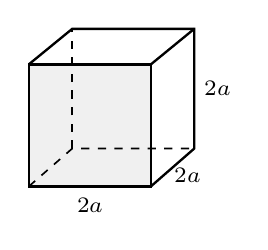
\begin{tikzpicture}[x=1cm, y=1cm, every node/.style={font=\footnotesize, text=black}]
      \draw[black, line width=0.9pt, fill=gray!12] (0,0) rectangle (1.55,1.55);
      \draw[black, line width=0.85pt] (1.55,0) -- (2.10,0.48) -- (2.10,2.00) -- (0.55,2.00) -- (0,1.55);
      \draw[black, line width=0.85pt] (1.55,1.55) -- (2.10,2.00);
      \draw[black, dashed, line width=0.6pt] (0,0) -- (0.55,0.48) -- (2.10,0.48);
      \draw[black, dashed, line width=0.6pt] (0.55,0.48) -- (0.55,2.00);
      \node at (0.78,-0.24) {$2a$};
      \node at (2.02,0.14) {$2a$};
      \node at (2.40,1.24) {$2a$};
    \end{tikzpicture}
  \end{minipage}\hfill
  \begin{minipage}[c]{14.3cm}
    $\bullet$ \textbf{១) គូបទ្រនុងប្រវែង $2a$ (ទំ.៥១)៖}\\[2pt]
    \hspace*{0.3cm}-- ផ្ទៃមុខខាងនីមួយៗ៖ $S = (2a) \times (2a) = (2a)^2 =$ \ansbox[2.2cm]\\[3pt]
    \hspace*{0.3cm}-- មាឌរបស់គូប៖ $V = (2a) \times (2a) \times (2a) = (2a)^3 =$ \ansbox[2.2cm]\\[3pt]
    $\bullet$ \textbf{២) បញ្ជាក់មេគុណ និងអថេរ (ទំ.៥២)៖} ឯកធា $-\dfrac{3}{4}ab^2x$ មានមេគុណ \ansbox[1.6cm] និងអថេរ \dotline[2.8cm] ។\\[3pt]
    $\bullet$ \textbf{៣) ប្រតិបត្តិទី ២ (ទំ.៥២ — គូស \ding{51} មុខឯកធា)៖} \quad
    \chkbox\ $\dfrac{1}{5}x^2y$ \quad
    \chkbox\ $3x^2 + 2$ \quad
    \chkbox\ $25 - \dfrac{2}{3}a^4bc^2$ \quad
    \chkbox\ $zx^2a^3b^4$
  \end{minipage}
\end{tcolorbox}

\vspace{4pt}
\textbf{សកម្មភាព ២ (\en{E2-B} — ៥ នាទី)៖ ឯកធាដូចគ្នា និងដឺក្រេនៃឯកធា (ទំ.៥២)}

\begin{tcolorbox}[
  enhanced, sharp corners, colback=white, colframe=black,
  boxrule=0.8pt, boxsep=2.5pt, top=4pt, bottom=4pt, left=6pt, right=6pt
]
  $\bullet$ \textbf{១) សង្កេតផ្នែកអថេរ៖} ឯកធា $-3xbc^2$ និង $\dfrac{2}{3}xbc^2$ មានផ្នែកអថេរ \dotline[2.2cm] ដូចគ្នា ហៅថា \textbf{ឯកធាដូចគ្នា} ។\\[3pt]
  $\bullet$ \textbf{២) ជ្រើសគូឯកធាដូចគ្នា៖} ក្នុងចំណោម $5x^2yz^3, \ \dfrac{7}{2}x^2cy^3, \ 5a^2bc^3, \ \dfrac{1}{2}x^2yz^3$ គូឯកធាដូចគ្នាគឺ \dotline[2.4cm] និង \dotline[2.4cm] ។\\[3pt]
  $\bullet$ \textbf{៣) គណនាដឺក្រេនៃឯកធា (ទំ.៥២)៖}\\[2pt]
  \hspace*{0.3cm}-- ឯកធា $3x = 3x^1$ មានដឺក្រេស្មើ \ansbox[1.3cm] \qquad
  -- ឯកធា $2xy = 2x^1y^1$ មានដឺក្រេ $1 + 1 =$ \ansbox[1.3cm]\\[3pt]
  \hspace*{0.3cm}-- ឯកធា $ax^2y = a^1x^2y^1$ មានដឺក្រេ $1 + 2 + 1 =$ \ansbox[1.3cm] \qquad
  -- ចំនួនថេរ $8 = 8x^0$ មានដឺក្រេស្មើ \ansbox[1.3cm]
\end{tcolorbox}

\vfill

% --- E3 Explain ---
\secstrip{ផ្នែកទី ៣ \enbf{(E3 - Explain)} ៖ និយមន័យគោល និងធនាគារហេតុផល \enbf{B\&W}}{រយៈពេល ៦ នាទី}

\begin{tcolorbox}[
  enhanced, sharp corners, colback=white, colframe=black,
  boxrule=0.85pt, boxsep=2.5pt, top=4pt, bottom=4pt, left=6pt, right=6pt
]
  $\bullet$ \textbf{១) ឯកធា៖} ជាកន្សោមពីជគណិតដែលមានតែប្រមាណវិធី \dotline[2.2cm] និងស្វ័យគុណដែលមាននិទស្សន្តជាចំនួនគត់ \dotline[3.0cm] ។\\[3pt]
  $\bullet$ \textbf{២) ឯកធាដូចគ្នា៖} ជាឯកធាដែលមានផ្នែក \dotline[2.3cm] ដូចគ្នា ។ \quad
  \textbf{៣) ដឺក្រេនៃឯកធា៖} ជាផលបូក \dotline[2.5cm] នៃអថេរទាំងអស់ ។\\[4pt]
  \tikz\draw[black, dashed, line width=0.5pt] (0,0) -- (18.4cm,0);\\[3pt]
  \fontsize{8.8pt}{13.0pt}\selectfont
  \textbf{ធនាគារហេតុផល (\en{Warrant Bank})៖} \quad
  \cnum{1} \textbf{ឯកធា៖} មានតែវិធីគុណនិងស្វ័យគុណគត់ $\ge 0$ \quad
  \cnum{2} \textbf{ឯកធាដូចគ្នា៖} ដូចគ្នាទាំងអថេរ ទាំងនិទស្សន្តតាមអថេរ\\
  \cnum{3} \textbf{និទស្សន្តលាក់មុខ៖} $a = a^1$ \quad
  \cnum{4} \textbf{ចំនួនថេរ៖} $c = cx^0\ (c\neq 0)$ ជាឯកធាដឺក្រេ $0$
\end{tcolorbox}

% ============================================================================
% ទំព័រទី ២៖ សន្លឹកកិច្ចការសិស្ស (ផ្នែកខាងខ្នង៖ E4 -> E5 -> កិច្ចការផ្ទះ)
% ============================================================================
\clearpage
\pagebanner{សន្លឹកកិច្ចការសិស្ស \enbf{(}៥\enbf{.}១\enbf{.}១\enbf{--}៥\enbf{.}១\enbf{.}៣ ឯកធា\enbf{)} \enbf{--} ផ្នែកខាងខ្នង}{ថ្នាក់ទី៨ \en{|} សៀវភៅគោល ទំ.៥២--៥៣, ៧២}

% --- E4 Elaborate ---
\secstrip{ផ្នែកទី ៤ \enbf{(E4 - Elaborate)} ៖ លំហាត់គំរូតារាងដឺក្រេ និងជ្រើសរើសឯកធាដូចគ្នា (ទំ.៥២--៥៣)}{រយៈពេល ១០ នាទី}

\begin{tcolorbox}[
  enhanced, sharp corners, colback=white, colframe=black,
  boxrule=0.8pt, boxsep=2.5pt, top=4pt, bottom=4pt, left=6pt, right=6pt
]
  \textbf{១) បំពេញតារាងមេគុណ អថេរ និងដឺក្រេនៃឯកធា (លំហាត់គំរូ ទំ.៥២--៥៣)៖}\\[4pt]
  {\renewcommand{\arraystretch}{1.42}
  \begin{tabular}{|C{3.2cm}|C{2.5cm}|C{3.6cm}|C{8.0cm}|}
    \hline
    \cellcolor{headgray}\textbf{ឯកធា} & \cellcolor{headgray}\textbf{មេគុណ} & \cellcolor{headgray}\textbf{អថេរ} & \cellcolor{headgray}\textbf{ផលបូកនិទស្សន្ត (ដឺក្រេនៃឯកធា)} \\ \hline
    $x^2yb^3$ & $1$ & $x, y, b$ & $2 + 1 + 3 =$ \dotline[1.6cm] \\ \hline
    $\dfrac{3}{4}a^2bc$ & \dotline[1.4cm] & \dotline[2.4cm] & $2 + 1 + 1 =$ \dotline[1.6cm] \\ \hline
    $x^3y^2$ & \dotline[1.4cm] & \dotline[2.4cm] & \dotline[3.4cm] \\ \hline
    $-3az^2y^3$ & \dotline[1.4cm] & \dotline[2.4cm] & \dotline[3.4cm] \\ \hline
  \end{tabular}}\\[5pt]
  \textbf{២) ប្រតិបត្តិទំ.៥២៖} ចូរជ្រើសរើសគូ\textbf{ឯកធាដូចគ្នា}ក្នុងចំណោម $\dfrac{1}{2}xy, \ -2x^2y, \ ay, \ 3ax, \ 2xy^2, \ xy$ គឺ៖ \ansbox[3.8cm]\\[3pt]
  \fontsize{8.8pt}{13.0pt}\selectfont
  \textbf{ឆ្លុះបញ្ចាំង (\en{EIA Looking-Back})៖} ហេតុអ្វី $-2x^2y$ និង $2xy^2$ មិនមែនជាឯកធាដូចគ្នា ទោះបីមានអក្សរ $x, y$ និងដឺក្រេ $3$ ស្មើគ្នាក៏ដោយ?\\[2pt]
  \textbf{ចម្លើយ៖} ព្រោះ \dotline[15.8cm] ។
\end{tcolorbox}

\vspace{4pt}

% --- E5 Evaluate ---
\secstrip{ផ្នែកទី ៥ \enbf{(E5 - Evaluate)} ៖ ប្រតិបត្តិ (ទំ.៥២--៥៣) សំណួរវិនិច្ឆ័យ \enbf{A--D} និងសំបុត្រចេញ}{រយៈពេល ១០ នាទី}

\begin{tcolorbox}[
  enhanced, sharp corners, colback=white, colframe=black,
  boxrule=0.8pt, boxsep=2.5pt, top=4pt, bottom=4pt, left=6pt, right=6pt
]
  \textbf{១) ប្រតិបត្តិទី ១ (ទំ.៥២)៖} ឯកធា $2\sqrt{3}yt^2$ មានមេគុណស្មើ \ansbox[1.8cm] អថេរគឺ \dotline[2.0cm] និងដឺក្រេស្មើ \ansbox[1.5cm] ។\\[4pt]
  \textbf{២) ប្រតិបត្តិ (ទំ.៥៣ ក, ខ, គ) — ចូរកំណត់អថេរ និងរកដឺក្រេនៃឯកធាខាងក្រោម៖}\\[3pt]
  \hspace*{0.3cm}$\bullet$ ក) $\dfrac{1}{2}xyz$៖ អថេរគឺ \dotline[2.2cm] \quad ដឺក្រេស្មើ \dotline[2.4cm] \qquad
  $\bullet$ ខ) $8x^3yz^2$៖ អថេរគឺ \dotline[2.2cm] \quad ដឺក្រេស្មើ \dotline[2.4cm]\\[3pt]
  \hspace*{0.3cm}$\bullet$ គ) $14$៖ អថេរគឺ \dotline[2.6cm] \quad ដឺក្រេស្មើ \ansbox[1.6cm] \quad (តាមលេខកូដហេតុផលទី \dotline[1.0cm])\\[4pt]
  \textbf{៣) បិទបេសកកម្ម \en{E1}៖} សិស្ស \dotline[1.0cm] ត្រឹមត្រូវ ព្រោះ $-3a^1z^2y^3$ មានដឺក្រេ $1 + 2 + 3 =$ \ansbox[1.5cm] ។
\end{tcolorbox}

\vspace{4pt}

\begin{tcolorbox}[
  enhanced, sharp corners, colback=white, colframe=black,
  boxrule=0.8pt, boxsep=2.5pt, top=4pt, bottom=4pt, left=6pt, right=6pt
]
  \textbf{៤) សំណួរវិនិច្ឆ័យ \en{A--D} (តើកន្សោមមួយណាជាឯកធាដូចគ្នានឹង $-5a^2b^3$? — គូសរង្វង់ រួចលើកម្រាមដៃ ១--៤)៖}\\[3pt]
  \textbf{\en{A.}} $-5a^3b^2$ \qquad\qquad
  \textbf{\en{B.}} $\dfrac{3}{4}b^3a^2$ \qquad\qquad
  \textbf{\en{C.}} $a^2 + b^3$ \qquad\qquad
  \textbf{\en{D.}} $-5a^2b^3c$\\[4pt]
  \tikz\draw[black, dashed, line width=0.5pt] (0,0) -- (18.4cm,0);\\[3pt]
  \textbf{៥) សំបុត្រចេញ ៦០ វិនាទី៖} ឯកធា $-7xy^4z$ មានមេគុណស្មើ \ansbox[1.6cm] អថេរគឺ \dotline[2.0cm] និងមានដឺក្រេស្មើ \ansbox[1.6cm] ។
\end{tcolorbox}

\vfill

% --- Homework ---
\begin{tcolorbox}[
  enhanced, sharp corners, colback=panelgray, colframe=black,
  boxrule=0.95pt, boxsep=2pt, top=3.5pt, bottom=3.5pt, left=6pt, right=6pt
]
  {\muol\fontsize{9.0pt}{13.0pt}\selectfont កិច្ចការផ្ទះ \enbf{(}សៀវភៅគោល ទំ.៥៣ និង ទំ.៧២ លេខ ១\enbf{)}}\\[2.5pt]
  \fontsize{8.8pt}{13.0pt}\selectfont
  $\bullet$ \textbf{១) ប្រតិបត្តិទំ.៥៣ (ង, ច, ឆ)៖} ចូរកំណត់អថេរនិងរកដឺក្រេនៃឯកធា៖ \quad ង) $21ab^4c$, \quad ច) $3x^2y^3z^4$, \quad ឆ) $axyz$ ។\\
  $\bullet$ \textbf{២) លំហាត់ \#1 (ទំ.៧២)៖} តើកន្សោមណាខ្លះជាឯកធា៖ $\dfrac{x^3}{3}, \ \sqrt{5}ax^2, \ \dfrac{7xy^2}{3}, \ x+2y, \ \dfrac{a}{x^2}, \ x(x+y)$? \textbf{អានមុន៖} ១.៤--១.៦ (ទំ.៥៣--៥៦) ។
\end{tcolorbox}

% ============================================================================
% ទំព័រទី ៣៖ ទំព័រគ្រូបង្រៀន (គំរូប្លង់ក្ដារខៀន ៣ ផ្នែក + ចម្លើយផ្ទៀងផ្ទាត់រហ័ស)
% ============================================================================
\clearpage
\pagebanner{ទំព័រគ្រូបង្រៀន ៖ ប្លង់ក្ដារខៀន \enbf{(}គ្មាន \enbf{LCD)} និងចម្លើយផ្ទៀងផ្ទាត់រហ័ស}{៥.១.១--៥.១.៣ ឯកធា (\en{ALG51})}

\secstrip{១. គំរូប្លង់បែងចែកក្ដារខៀន ៣ ផ្នែក សម្រាប់ថ្នាក់រៀនគ្មាន \enbf{LCD}}{សម្រាប់គ្រូប្រើដីស/ហ្វឺត}

\begin{center}
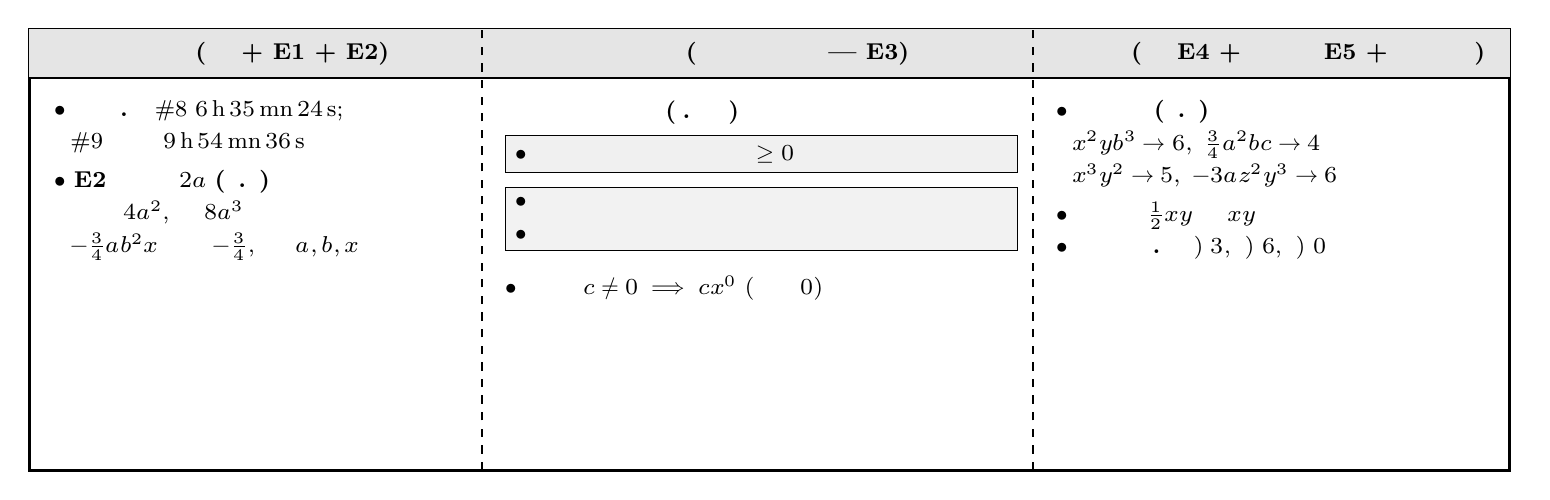
\begin{tikzpicture}[x=1cm, y=1cm, every node/.style={font=\fontsize{8.3pt}{11.8pt}\selectfont, text=black}]
  \draw[black, line width=1.1pt] (0,0) rectangle (18.8,5.60);
  \fill[gray!20] (0,4.98) rectangle (18.8,5.60);
  \draw[black, line width=0.7pt] (0,4.98) -- (18.8,4.98);
  \draw[black, dashed, line width=0.7pt] (5.75,0) -- (5.75,5.60);
  \draw[black, dashed, line width=0.7pt] (12.75,0) -- (12.75,5.60);

  \node at (2.875,5.29) {\textbf{ផ្នែកឆ្វេង (កំណែ + \en{E1} + \en{E2})}};
  \node at (9.25,5.29) {\textbf{ផ្នែកកណ្ដាល (ខ្លឹមសារគោលរក្សាទុក — \en{E3})}};
  \node at (15.775,5.29) {\textbf{ផ្នែកស្ដាំ (គំរូ \en{E4} + ប្រតិបត្តិ \en{E5} + កិច្ចការផ្ទះ)}};

  % Left
  \node[anchor=north west, text width=5.35cm] at (0.20,4.82) {%
    $\bullet$ \textbf{កំណែ ទំ.៥០៖} \#8 $6\unit{h}\,35\unit{mn}\,24\unit{s}$;\\
    \hspace*{0.2cm}\#9 ជួបម៉ោង $9\unit{h}\,54\unit{mn}\,36\unit{s}$\\[2pt]
    $\bullet$ \textbf{\en{E2} គូបទ្រនុង $2a$ (ទំ.៥១)៖}\\
    \hspace*{0.2cm}ផ្ទៃមុខ $4a^2$, មាឌ $8a^3$\\
    \hspace*{0.2cm}$-\tfrac{3}{4}ab^2x$៖ មេគុណ $-\tfrac{3}{4}$, អថេរ $a,b,x$
  };

  % Center
  \node[anchor=north west, text width=6.65cm] at (5.92,4.82) {%
    {\muol\fontsize{8.5pt}{12pt}\selectfont មេរៀនទី៥៖ កន្សោមពីជគណិត \enbf{(}១\enbf{.} ឯកធា\enbf{)}}\\[3pt]
    \tikz\node[draw=black, fill=gray!12, inner sep=3.5pt, text width=6.25cm]{%
      $\bullet$ \textbf{ឯកធា៖} មានតែវិធីគុណ និងស្វ័យគុណគត់ $\ge 0$
    };\\[4pt]
    \tikz\node[draw=black, fill=gray!10, inner sep=3.5pt, text width=6.25cm]{%
      $\bullet$ \textbf{ឯកធាដូចគ្នា៖} មានផ្នែកអថេរដូចគ្នា\\
      $\bullet$ \textbf{ដឺក្រេឯកធា៖} ផលបូកនិទស្សន្តនៃអថេរទាំងអស់
    };\\[4pt]
    $\bullet$ ចំនួនថេរ $c \neq 0 \implies c x^0$ (ដឺក្រេ $0$)
  };

  % Right
  \node[anchor=north west, text width=5.8cm] at (12.92,4.82) {%
    $\bullet$ \textbf{តារាងដឺក្រេ (ទំ.៥៣)៖}\\
    \hspace*{0.2cm}$x^2yb^3 \to 6, \ \tfrac{3}{4}a^2bc \to 4$\\
    \hspace*{0.2cm}$x^3y^2 \to 5, \ -3az^2y^3 \to 6$\\[2pt]
    $\bullet$ \textbf{គូដូចគ្នា៖} $\tfrac{1}{2}xy$ និង $xy$\\
    $\bullet$ \textbf{ប្រតិបត្តិទំ.៥៣៖} ក) $3$, ខ) $6$, គ) $0$
  };
\end{tikzpicture}
\end{center}

\vspace{4pt}
\secstrip{២. ចម្លើយផ្ទៀងផ្ទាត់រហ័សសម្រាប់សន្លឹកកិច្ចការសិស្ស \enbf{(}ទំព័រ ១ និង ទំព័រ ២\enbf{)}}{\en{Answer Key}}

\begin{tcolorbox}[
  enhanced, sharp corners, colback=white, colframe=black,
  boxrule=0.8pt, boxsep=2pt, top=4pt, bottom=4pt, left=6pt, right=6pt
]
  \fontsize{9.0pt}{13.5pt}\selectfont
  $\bullet$ \textbf{ផ្នែក \en{E1}៖} \textbf{សិស្ស ខ} ត្រឹមត្រូវ ព្រោះ $a = a^1$ នាំឱ្យដឺក្រេស្មើ $1 + 2 + 3 = 6$ ។\\[2pt]
  $\bullet$ \textbf{ផ្នែក \en{E2}៖} \textbf{សកម្មភាព ១៖} $4a^2, \ 8a^3$; មេគុណ $-\frac{3}{4}$ អថេរ $a, b, x$; ឯកធាគឺ $\frac{1}{5}x^2y$ និង $zx^2a^3b^4$ ។ \textbf{សកម្មភាព ២៖} $5x^2yz^3$ និង $\frac{1}{2}x^2yz^3$; ដឺក្រេ $1, \ 2, \ 4$ ។\\[2pt]
  $\bullet$ \textbf{ផ្នែក \en{E4}៖} តារាងដឺក្រេ៖ $6$; អថេរ $a,b,c$ ដឺក្រេ $4$; អថេរ $x,y$ ដឺក្រេ $3+2=5$; អថេរ $a,z,y$ ដឺក្រេ $1+2+3=6$ ។ គូដូចគ្នា៖ $\frac{1}{2}xy$ និង $xy$ ។\\[2pt]
  $\bullet$ \textbf{ផ្នែក \en{E5}៖} ១) មេគុណ $2\sqrt{3}$ អថេរ $y,t$ ដឺក្រេ $3$; ២) ក) $3$, ខ) $6$, គ) $0$; ៣) សិស្ស ខ ($6$); ៤) \textbf{ជម្រើស \en{B}} ($\frac{3}{4}b^3a^2$); ៥) មេគុណ $-7$ ដឺក្រេ $6$ ។
\end{tcolorbox}

\vspace{4pt}
\secstrip{៣. ចម្លើយលម្អិតនៃកិច្ចការផ្ទះ \enbf{(}សម្រាប់ផ្ទៀងនៅដើមម៉ោងបន្ទាប់ ៥\enbf{.}១\enbf{.}៤\enbf{)}}{សៀវភៅគោល ទំ.៥៣, ៧២}

\begin{tcolorbox}[
  enhanced, sharp corners, colback=white, colframe=black,
  boxrule=0.8pt, boxsep=2pt, top=4pt, bottom=4pt, left=6pt, right=6pt
]
  \fontsize{8.8pt}{13.2pt}\selectfont
  $\bullet$ \textbf{១) ប្រតិបត្តិទំ.៥៣ (ង, ច, ឆ)៖} ង) $21ab^4c$ មានអថេរ $a, b, c$ និងដឺក្រេ $1+4+1 = \mathbf{6}$; \quad ច) $3x^2y^3z^4$ មានអថេរ $x, y, z$ និងដឺក្រេ $2+3+4 = \mathbf{9}$; \quad ឆ) $axyz$ មានអថេរ $a, x, y, z$ និងដឺក្រេ $1+1+1+1 = \mathbf{4}$ ។\\[2pt]
  $\bullet$ \textbf{២) លំហាត់ \#1 (ទំ.៧២)៖} កន្សោមដែលជា\textbf{ឯកធា}គឺ $\mathbf{\dfrac{x^3}{3}}$ ($= \frac{1}{3}x^3$), $\mathbf{\sqrt{5}ax^2}$ និង $\mathbf{\dfrac{7xy^2}{3}}$ ($= \frac{7}{3}xy^2$) ។ រីឯ $x+2y$ និង $x(x+y) = x^2+xy$ ជាពហុធា (ទ្វេធា) ហើយ $\dfrac{a}{x^2}$ ជាកន្សោមសនិទាន (មានអថេរនៅភាគបែង) មិនមែនជាឯកធាឡើយ ។
\end{tcolorbox}

\end{document}
